\makeatletter
\def\@makechapterhead#1{%
  \vspace*{10\p@}%
  {\parindent \z@ \raggedleft \normalfont
    \ifnum \c@secnumdepth >\m@ne
      \if@mainmatter
        \LARGE\bfseries \@chapapp\space \thechapter
	\vskip 4pt
        \hrule height 2pt
        \par\nobreak
        \vskip 5\p@
      \fi
    \fi
    \interlinepenalty\@M
    \huge \bfseries #1\par\nobreak
\vskip 5pt

\hrule height 2pt   
 \vskip 10\p@  
  }}
\makeatother

\setcounter{chapter}{7}
\chapter{Communication Systems}\label{chap8}
\addtocontents{toc}{\protect\contentsline{chapter}{\protect Chapter \numberline{\thechapter.}
Communication Systems}{\thepage--\pageref{8end}}}  

\section{Introduction}\label{sec8.1}%% 8.1

In its basic electric sense, the term communication refers to the
sending and receiving of an information from one point to another
point. Basically, communication systems are of two types.
\begin{itemize}
\item[(i)] Wire communication: i.e., where communication is done
  through a wire. e.g., cable TV, wire telephony etc.

\item[(ii)] Wireless communication: i.e., where communication is done
  without using a wire. In this system high frequency carrier wave is
  used. It is also called radio or career communication. e.g.,  radio,
  TV, radar, radio radio telephony etc.
\end{itemize}

\section{Elements of Communication systems}\label{sec.8.2}%%% 8.2

Fig~\ref{fig8.1} shows the bank elements or block diagram of a communication
system.
\begin{figure}[H]
\centering
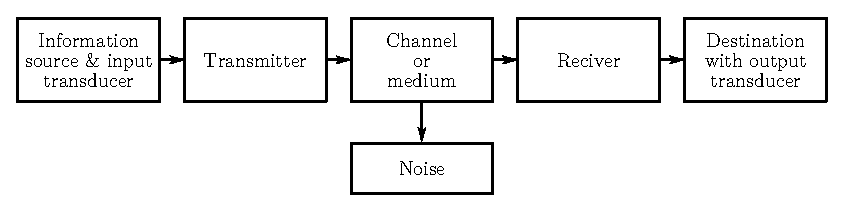
\includegraphics{chap8/fig8.1.eps}
\caption{Elements of a communication system.}\label{fig8.1}
\end{figure}

The message produced by an information source is not electrical in
nature. Hence an input transducer is required for converting the
message into a time varying electrical signal called message
signal. At the destination point, another transducer converts the
electrical signal into the appropriate message signal.

\eject

\heading{The Transmitter:} The transmitter couples the input message
signal to the channel or medium. It is a collection of electronic
circuits designed to convert the message into a signal suitable for
transmission over a given channel. The basic operation, performed by
the transmitter include amplification, filtering and
modulation. Amplification is required because the electrical signal
obtained from the output of the input transducer may be very
weak. Filtering is done to restrict the frequencies of the signal. The
most important is the modulation which match the properties of the
signal to be transmitted to the channel through the use of a high
frequency carrier wave.

\heading{The Channel and Noise Source:} The term channel implies the
medium through which the message travels from transmitter to
receiver. Channels may be wired (wire communication) or non-wired
(radio communicate). Some examples for wired channels are telephone
lines, coaxial cable etc. and for non-wired channels are air, vacuum,
seawater, etc.

During the process of transmission and reception, the signal gets
deteriorated due to superimposition of noise into it. The noise can be
classified into two broad groups.
\begin{itemize}
\item[(i)] noise whose sources are external to the receiver and 

\item[(ii)] noise created within the receiver itself.
\end{itemize}

If the noise gets superimposed on the signal severely, the signal to
noise ratio becomes so poor that the signal becomes unintelligible and
hence useless. 

Infact, noise may get added to the signal at any point in the
communication system. However, the noise has its greatest damaging
effect when the signal is weakest.

\heading{The Receiver:} The main functions of the receiver is to
extract the input message signal from the degraded version of the
transmitted signal coming from the channel. The receiver performs this
operation through the process called demodulation, the reverses  of
the transmitter's modulation process...

\section{Modulation}\label{sec8.3}

Modulation is defined as the process by which some characteristics of
a high frequency sinusoidal wave (the carrier wave) is varied in
accordance with the instantaneous value of the modulating signal
(message signal). The frequency of the carrier is called carrier
frequency and the frequency of the modulating  signal is called
modulation frequency. Usually, the modulating frequency is
considerably lower than the carrier frequency.

Let the high frequency carrier wave is represented by the expression,
\begin{equation}
 v_{\rmc(\rmt)} = \rmE_c \sin (\omega_{\rmc}{\rmt} + \phi_{\rmc} )\label{eq8.1}
\end{equation}
\begin{tabbing}
where ~$v_{\rmc(\rmt)}$ \= = \= instantaneous value of the carrier wave
(V)\\[4pt]
\hspace{1.1cm} ~$E_{\rmc}$ \> = \> amplitude of the carrier wave (V)\\[4pt]
\hspace{1.1cm} ~$\omega_{\rmc}$ \> = \> $2 \pi f_{\rmc}$ = angular frequency of the
carrier wave (rad/sec)\\[4pt]
\hspace{1.13cm} ~$f_{\rmc}$ \> = \> frequency of the carrier wave (Hz)\\[4pt]
\hspace{1.13cm} ~$\phi_{\rmc}$ \> = \> phase angle (rad) and ~t = time.
\end{tabbing}

The modulation process varies any one of these three quantities
(E$_{\rmc}$, $\omega_{\rmc}$ and $\phi_{\rmc}$) of the carrier wave in
accordance with the instantaneous value of the modulating signal
(message signal). If amplitude of  the carrier wave E$_{\rmc}$ is
varied in accordance with the instantaneous value of the modulating
signal, then it is called amplitude modulation (AM). If frequency
$\omega_{\rmc}$ or f$_{\rmc}$ of the carrier wave is varied in
accordance with the instantaneous value of the modulating signal, then
it is called frequency modulation (FM). Similarly, if the phase of the
carrier wave is varied in accordance with the instantaneous value of
the modulating signal, then it is called phase modulation (PM). FM and
PM are grouped together under the heading angular modulation. It is
possible to produce amplitude, frequency and phase modulation of the
carrier wave by varying all the three parameters E$_{\rmc}$ f$_{\rmc}$
or $\omega_{\rmc}$ and $\phi_{\rmc}$ simultaneously. But in commercial
radio communication, only one type of modulation is done excluding the
other two.

Table 8.1.  gives the earrier frequency bands used for various
communication systems. 

\begin{table}[H]
\caption{Frequency bands for various communication systems.}\label{tab8.1}
\begin{tabular}{c|l|l}
\hline
{\bf Sl.No.} & \multicolumn{1}{c|}{\bf Frequency Band} & \multicolumn{1}{c}{\bf Applications}\\
\hline
1. & Very low frequency (3 kHz - 30 kHz) & Long distance
communications\\[-0.1cm]
& & like submarine communication,\\[-0.1cm]
& & navigation etc.\\[0.2cm]
2. & Low frequency (30 kHz - 300 kHz) & Radio navigation \\[0.2cm]
3. & Medium frequency  (300 kHz - 3 MHz) & AM broadeast\\[0.2cm]
4. & High frequency (3 MHz - 30 MHz) & Commercial short - wave\\[-0.1cm]
& & broadcasting like FM\\[-0.1cm]
& & television. \\[0.2cm]
5. & Very High frequency (30 MHz - 300 MHz) & TV and FM broadcast\\[0.2cm]
6. & Ultra High frequency (300 MHz - 3 GHz) & Sattelite
communication, \\[-0.1cm]
& & cellular phones, personal\\[-0.1cm]
& & communication systems etc.\\[0.2cm]
7. & Super High frequency (3 GHz - 30 GHz) & Radar, satellite \\[-0.1cm]
& & communication etc.\\
\hline
\end{tabular}
\end{table}

\section{Need for Modulation}\label{sec8.4}

Sometimes the question may arise that why high frequency carrier wave
is required to carry the low frequency modulating signal (message
signal) from one place to another? Why not we transmit the message
signal directly?

If the channel in which the message signal is to be transmitted is low
pass in nature, the low pass message signal may be transmitted over
the channel without modulation. Such type of signal transmission is
called baseband communication. But the majority of the practical
channels have bandpass characteristics. Therefore modulation is
necessary for translating the lowpass message signal spectrum to match
the bandpass channel characteristics. The matching of the message
signal to the channel characteristics results in several important
aspects as given below.
\begin{itemize}
\item[(i)] Practicability of Antinna : When free space is a
communication channel, antenna radiate and receive the signals. But
the antenaa operate effectively only when their dimensions are of the
order of the magnitude of the wavelength of the signal to be
transmitted. For example, a signal of 1 KHz corresponds to a
wavelength of 3,00,000 mtrs.      
\begin{tabbing}
(~$\therefore ~v = {\rmf} \lambda$ where ~$v$ \= = \= velocity of the
wave in free space = 3 $\times$ 10 m)\\[4pt]
\hspace{2.67cm} $f$ \> = \>  frequency of the wave (Hz)\\[4pt]
\hspace{2.77cm}$\lambda$ \> = \> wave length of the wave (m).
\end{tabbing}

Therefore to transmit a 1 kHz signal we need an antenaa of length
3,00,000 mtrs, which is highly impractical. The required dimenssions
may be reduced to the point  of practicability by translating the
message signal to high frequency band by modulation.

\item[(ii)] Frequency multiplexing : If more than are signal utilizes
a single channel, modulation may be used to translate different
signals to different spectral location, thus enabling the receiver to
select the desired signal at the receiving  end by using appropriate
bandpass filters.

\item[(iii)] Narrowbanding : Let us assume that the message signal in
the frequency range to be transmitted extends from 50 Hz to 10$^4$
Hz. The ratio of highest frequency to lowest frequency is
$\dfrac{10^4 ~\rmk \rmH \rmz}{50 ~\rmH \rmz} = 200$. Therefore, an
antenna suitable for the use at one end of the frequency range would
be entirely too short or too long for the other end. Suppose that the
frequency is translated, such that it occupies the frequency range
from $(10^6 + 50)$ Hz to $(10^6 + 10^4)$ Hz, the ratio of highest to
lowest frequency decreases to $\dfrac{(10^6+ 50)}{10^6+ 10^4} =
0.99$. Thus to process of modulation may be used to change a wideband
signal into a narrow band signal which can be more conveniently
processed. 

\item[(iv)] Reduced noise or Interference : It is possible to minimize
the effects of noise and interference by using certain types of
modulation schemes. 
\end{itemize}

\section{Amplitude Modulation}\label{sec8.5}

In amplitude modulation (AM), the amplitude of the high frequency
carrier signal is varied in accordance with the instantaneous value of
the modulating signal (message signal).

\heading{Expression for amplitude modulated signal :}
\smallskip

Let the carrier wave be given by the expression,
\begin{equation}
\rme_{\rmc}(\rmt) = \rmE_{\rmc} \sin \omega_{\rmc} \rmt.\label{eq8.2}
\end{equation}

In Eqn.~\eqref{eq8.2}, the phase angle $\phi_{\rmc}$ has been taken as
zero because it doesnot play any role in the modulation process.

In AM, the amplitude of the unmodulated carrier wave will have to be
made proportional to the instantaneous value of the modulating signal
(message signal) ~${\rme}_{\rmm}(\rmt) =
{\rmV}_{\rmm} \sin \omega_{\rmm} {\rmt}$.

Let e(t) be the instantaneous value of the modulated signel.
\begin{align}
\rme(\rmt) & = \rmE \sin \omega_{\rmc} \rmt\label{eq8.3}\\[3pt]
\text{where } \qquad \rmE & = \rmE_{\rmc} + \rme_{\rmm} (\rmt) \qquad \label{eq8.4}
\end{align}

Substituting Eqn.~\eqref{eq8.4} in Eqn.~\eqref{eq8.3},
\begin{align}
\rme(\rmt) & = (\rmE_\rmc + \rme_\rmm(\rmt)) \sin \omega_\rmc \rmt\label{eq8.5}\\[3pt]
& = (\rmE_\rmc + \rmE_\rmm \sin \omega_\rmm \rmt) \sin \omega_\rmc \rmt \label{eq8.6}\\[3pt]
& = \rmE_\rmc (1+\rmE_\rmm/\rmE_\rmc \sin \omega_\rmm \rmt)  \sin \omega_\rmc \rmt\notag \\[3pt]
\rme(\rmt) & = \rmE_\rmc (1+ \rmm \sin \omega_\rmm\rmt) \sin \omega_\rmc \rmt\label{eq8.7}
\end{align}
where $\rmm=\rmE_\rmm/\rmE_\rmc$ is called \textit{modulation index}
or \textit{depth of modulation} $(0 < n \leq 1)$. Eqn.~\eqref{eq8.7}
is known as \textit{AM wave equation.}
\begin{figure}[H]
\centering
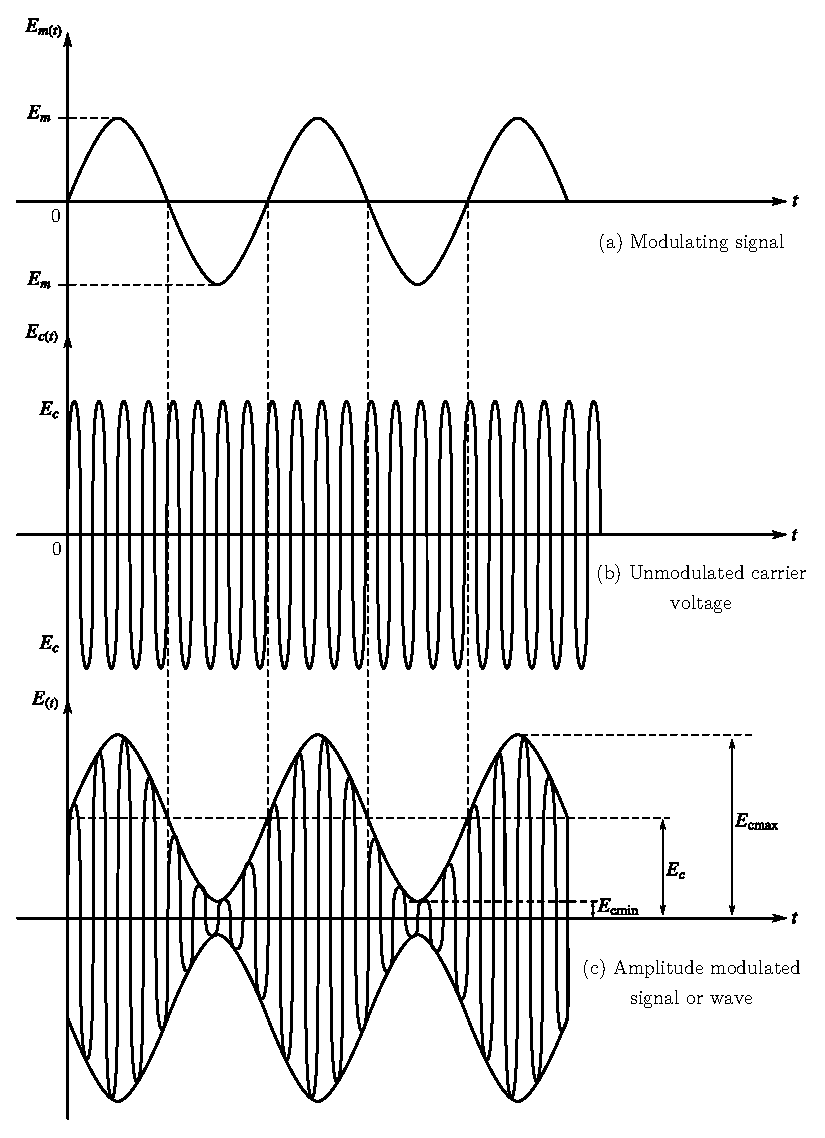
\includegraphics[scale=0.88]{chap8/fig8.2.eps}
\caption{Waveform of amplitude modulated carrier wave.}\label{fig8.2}
\end{figure}

\vskip -.6cm

Fig.~\ref{fig8.2}(a) shows the waveform of modulating
signal. Fig.~\ref{fig8.2}(b) shows the waveform of high frequency
unmodulated carrier wave and Fig.~\ref{fig8.2}(c) shows the waveform of
amplitude modulated signal.

From Fig.~\ref{fig8.2}(c), 
\begin{align}
\rmE_\rmm &=\frac{\rmE_{\rmc \max}
- \rmE_{\rmc \min}}{2}\label{eq8.8}\\[4pt]
\text{and} \qquad \rmE_\rmc & = \rmE_{\rmc \max} - \rmE_\rmm \label{eq8.9}
\end{align}
Substituting Eqn.~\eqref{eq8.8} in Eqn.~\eqref{eq8.9},
$$
\therefore \rmE_\rmc = \frac{\rmE_{\rmc \max} + \rmE_{\rmc \min}}{2}
$$
$\therefore$ ~\text{Modulation index ~~~}
\begin{align}
 \rmm  & = \dfrac{\rmE_\rmm}{\rmE_\rmc}
= \dfrac{\rmE_{\rmc\max} - \rmE_{\rmc \min}/2}{(\rmE_{\rmc\max} + \rmE_{\rmc\min})/2}\notag\\[0.2cm]
\therefore~ \rmm & = \dfrac{\rmE_{\rmc \max} + \rmE_{\rmc \min}}{\rmE_{\rmc \max}
+ \rmE_{\rmc \min}}\label{eq8.10}
\end{align}

Eqn.~\eqref{eq8.10} is the standard equation to find the modulation
index from the AM wave.

\subsection{Spectrum Power}\label{sec8.5.1} 
From Eqn.~\eqref{eq8.7}, 
\begin{align}
\rme(\rmt) & = \rmE_\rmc (1+\rmm\sin \omega_\rmm \rmt) \sin \omega_\rmc \rmt\notag\\[4pt]
& = \rmE_\rmc \sin \omega_\rmc \rmt + \rmm \rmE_\rmc \sin \omega_\rmm \rmt \sin \omega_\rmc \rmt\notag \\[4pt]
& = \rmE_\rmc \sin \omega_\rmc \rmt +  \frac{\rmm\rmE_\rmc}{2} \cos
(\omega_\rmc -\omega_\rmm)\rmt - \frac{\rmm \rmV_\rmc}{2} \cos (\omega_\rmc
+ \omega_\rmm) \rmt \label{eq8.11}
\end{align}

Thus equation of amplitude modulated wave contains three terms. The
first term is indentical to Eqn.~\eqref{eq8.2} and represents the
unmodulated carrier wave. The two additional terms produced are the
two sidebands. The frequency of lower sideband (LSB) is $\omega_\rmc
-\omega_\rmm$ and the frequency of upper side band (USB) is $\omega_\rmc
+ \omega_\rmm$. Thus the bandwidth required for AM signal is twice the
frequency of the modulating signal, i.e., $(\omega_\rmc + \omega_\rmm)
- (\omega_\rmc - \omega_\rmm) = 2 \omega_\rmm$.

\eject

Fig.~\ref{eq8.3} show frequency spectrum of amplitude modulated
wave.
\begin{figure}[H]
\centering
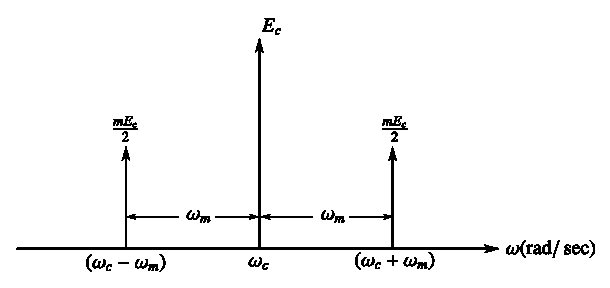
\includegraphics{chap8/fig8.3.eps}
\caption{Frequency specturm of AM wave}\label{fig8.3}
\end{figure}

So far, we have assumed that the modulating signal has a single
frequency tone. But practically, the modulating signal is a complex
waveform i.e., the modulating signal consists of a band of frequencies
of different amplitudes. Each frequency term in this modulating signal
produces a pair of sideband terms on modulation. Thus the entire
modulating signal produces two sidebands symmetrically placed about
the carrier as shown in Fig.~\ref{fig8.4}. Here $\omega_1$ and
$\omega_2$ are the lowest and highest frequencies in the modulating
signal.
\begin{figure}[H]
\centering
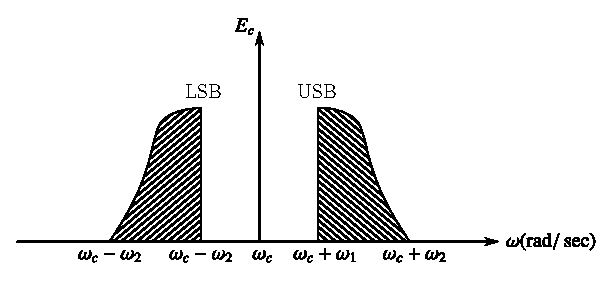
\includegraphics{chap8/fig8.4.eps}
\caption{Frequency specturm of amplitude modulated wave by complex
modulating signal}\label{fig8.4}
\end{figure}

\subsection{Power relations in AM wave}\label{sec8.5.2}
We have seen that the carrier component of the amplitude modulated
wave has the same amplitude as the unmodulated carrier wave. In
addition to this, the AM wave contains two sideband
components. Therefore, the modulated wave contains more power than the
carrier wave before modulation. Further, since the amplitude of the
sidebands depends on the modulation index m, the total power in the
modulated wave will also depend on the modulation index. The total
power in the amplitude modulated wave is 
\begin{align}
\rmP_\rmt & = \rmP_\rmc + \rmP_{\text{ LSB}} + \rmP_{\text{ USB}} \label{eq8.12}\\[4pt]
& = \frac{\rmE^2_{\text{ carr}}}{\rmR} + \frac{\rmE^2_{\text{
LSB}}}{\rmR} + \frac{\rmE^2_{\text{ USB}}}{\rmR} \label{eq8.13}
\end{align}
\begin{tabbing}
\hspace{1cm} where ~ $E_{\text{ carr}}$ \= = \= rms value of carrier wave\\[3pt]
\hspace{2cm} ~ $E_{\text{~LSB}}$ \> = \> rms value of LSB component\\[3pt]
\hspace{2cm} ~ $E_{\text{~USB}}$ \> = \> rms value of USB component
\end{tabbing}

The first term in Eqn.~\eqref{eq8.12} is the unmodulated carrier power
and is given by
\begin{equation}
\rmP_\rmc = \rmE^2_{\text{ carr}} = \frac{(\rmE_\rmc/\sqrt{2})^2}{\rmR} = \frac{\rmE^2_\rmc}{2\rmR} \label{eq8.14}
\end{equation}

Similarly, $\rmP_{\text{ LSB}} = \rmE_{\text{ USB}} = \dfrac{{\rmE}^2_{\text{ LSB}}}{\rmR}$
\begin{align}
& = \left(\frac{\rmm \rmE_\rmc/2}{\sqrt{2}} \right)^2 \times \frac{1}{\rmR}\notag\\[4pt]
\therefore\quad  \rmE_{\text{ LSB}} & = \rmE_{\text{ USB}} = \frac{\rmm^2}{4} \cdot \frac{\rmE^2_\rmc}{2\rmR}\label{eq8.15}
\end{align}

Substituting Eqn.~\eqref{eq8.14} and \eqref{eq8.15} in Eqn.~\eqref{eq8.12},
\begin{align}
\therefore ~ \text{Total Power} ~  \rmP_\rmt  & = \frac{\rmE^2_\rmc}{2\rmR}
+ \frac{\rmm^2}{4} \frac{\rmE^2_\rmc}{2\rmR}
+ \frac{\rmm^2}{4} \cdot \frac{\rmE^2_\rmc}{2\rmR}\notag\\[4pt]
& = \rmP_\rmc + \frac{\rmm^2}{4} + \rmP_\rmc + \frac{\rmm^2}{4} \rmP_\rmc \notag\\[4pt]
\therefore ~~ \rmP_\rmt & = \rmP_\rmc \left[1 + \frac{\rmm^2}{2} \right]\label{eq8.16}
\end{align}

Eqn.~\eqref{eq8.16} relates the total power in the amplitude modulated
wave to the unmodulated carrier power $\rmP_\rmc.$

From Eqn.~\eqref{eq8.16}, it reveals that the maximum power in the AM
is $\rmP_\rmt = 1.5$ $\rmP_\rmc$ because $0< \rmm \leq 1$.

\eject

\noindent
{\textit{\textbf{Current relations in AM wave}}}

Let $\rmI_\rmc$ be the rms value of unmodulated current and $\rmI_\rmt$ be
the rms value of total or modulated current of an AM transmitter. Let
R be the resistance into which these current flows, then
\begin{align}
\frac{\rmP_\rmt}{\rmp_\rmc} &= \frac{\rmI_\rmt^2 \rmR}{\rmI^2_\rmc \rmR}
= \left(\frac{\rmI_\rmt}{\rmI_\rmc} \right)^2 = 1 + \frac{\rmm^2}{2}\notag\\[3pt]
\therefore ~ \rmI_\rmt & = \rmI_\rmc \sqrt{1+ \frac{\rmm^2}{2}}\label{eq8.17}
\end{align}

\medskip
\noindent
{\textit{\textbf{Modulation by several sine waves}}}

In practice, carrier is modulated by several sine waves
simultaneously. In this case, there are two methods to compute total
modulation index $\rmm$. Then, this value of $\rmm$ is substituted in
Eqn.~\eqref{eq8.16} to compute the total power.


\begin{method}%% I
Let $\rmE_1$, $\rmE_2$, $\rmE_3$ etc. be the amplitude of simultaneous
modulating signal. Then the total modulating voltage $\rmE_\rmt$ equals the
square root of the sum of the squares of the individual modulating
voltages.
\begin{equation}
\text{i.e., } \rmE_\rmt =\sqrt{\rmE^2_1 + \rmE^2_2 + \rmE^2_3 + \ldots} \label{eq8.18}
\end{equation}

Dividing by $\rmE_\rmc$ on both the sides,
\begin{align}
\frac{\rmE_\rmt}{\rmE_\rmc} & = \frac{\sqrt{\rmE^2_1 + \rmE^2_2 + \rmE^2_3 + \cdots}}{\rmE_\rmc}\notag\\[3pt]
\frac{\rmE_\rmt}{\rmE_\rmc} & = \sqrt{\left(\frac{\rmE_1}{\rmE_\rmc} \right)^2 + \left(\frac{\rmE_2}{\rmE_\rmc} \right)^2
+ \left(\frac{\rmE_3}{\rmE_\rmc} \right)^2 + \cdots}\notag\\[3pt]
\therefore ~ \rmm & =  \sqrt{\rmm^2_1 + \rmm^2_2 + \rmm_3^2 + \cdots } \label{eq8.19}
\end{align}
\end{method}

\begin{method}%%% II
Considering Eqn.~\eqref{eq8.16},
\begin{align}
\rmP_\rmt & = \rmP_\rmc \left(1+ \frac{\rmm^2}{2} \right)\notag\\
\rmP_\rmt & = \rmP_\rmc + \rmP_\rmc  \cdot \frac{\rmm^2}{2}\notag\\
\rmP_\rmt & = \rmP_\rmc + \rmP_{\text{ SB}} \label{eq8.20}
\end{align}
where $\rmP_{\rmS\rmB}$ = Total sideband power and is given by,
\begin{equation}
\rmP_{\rmS\rmB} = \rmP_\rmc \cdot \frac{\rmm^2}{2}\label{eq8.21}
\end{equation}

When several sinewaves simultaneously modulate the carrier wave; the
carrier power $\rmP_\rmc$ remains unaltered. But the sideband power $\rmP_{\rmS\rmB}$
is the sum of the individual sideband powers. Then,
\begin{equation}
\rmP_{\rmS\rmB} = \rmP_{\rmS\rmB1} + \rmP_{\rmS\rmB2} + \rmP_{\rmS\rmB3} + \ldots\label{eq8.22}
\end{equation}

Substituting Eqn.~\eqref{eq8.21} in Eqn.~\eqref{eq8.22},
\begin{align}
\frac{\rmP_\rmc \rmm^2}{2} & = \frac{\rmP_\rmc \rmm^2_1}{2} + \frac{\rmP_\rmc \rmm^2_2}{2}
+ \frac{\rmP_\rmc \rmm^2_3}{2} + \cdots \notag\\
\therefore ~ \rmm & = \rmm_1^2 + \rmm^2_2 + \rmm_3^2 + \cdots \label{eq8.23}
\end{align}

It must be noted that the total modulation index must not exceed unity
or else distortion will result. In case of amplitude modulation of
carrier wave by several sinewaves simultaneously, the bandwidth
required is twice the highest modulating frequency.
\end{method}

\begin{center}
\rule{4cm}{1pt}\\
{\bf\Large Problems}\\[-3pt]
\rule{4cm}{1pt}
\end{center}

\begin{problem}\label{prob8.1}
A sinusoidal carrier wave of frequency 10 MHz and amplitude 200 V is
amplitude modulated by a sinusoidal wave of frequency 10 kHz producing
40\% modulation. Calculate the frequency and amplitude of upper and
lower sidebands.
\end{problem}

\begin{solution}
Given ~$\rmf_\rmc = 10$ MHz, ~~$\rmE_\rmc = 200$, ~~$\rmf_\rmm =10$
kHz, ~~$\rmm = 0.4$

\smallskip
\begin{tabbing}
Amplitude of upper and lower sideband \= = \= $\dfrac{\rmm\rmE_\rmc}{2}$\\[0.2cm]
\> = \> $\dfrac{0.4 \times 200}{2}$\\[0.2cm]
\> = \> 40 V
\end{tabbing}
\begin{tabbing}
Frequency of USB \= = \= $\rmf_\rmc + \rmf_\rmm = 10 \times 10^6 + 10 \times 10^3$\\[0.1cm]
\> = \> 10010 kHz\\[0.1cm]
Frequency of LSB \> = \> $\rmf_\rmc - \rmf_\rmm = 10 \times 10^6 -10 \times 10^3$\\[0.1cm]
\> = \> 9990 kHz
\end{tabbing}
\end{solution}

\begin{problem}\label{prob8.2}
The tuned circuit of the oscillator in a simple AM transmitter uses a
coil of 20 $\mu$H and shunt capacitor of value 0.8 nF. If the
oscillator output is modulated by audio frequencies upto 10 kHz, what
is the frequency range occupied by the sidebands.
\end{problem}

\begin{solution}
Given $\rmL = 20 ~\mu\rmH$, ~~C=0.8 nF

Maximum value of audio frequency $\rmf_\rmm$ = 10 KHz
\begin{tabbing}
Frequency of oscillator output $\rmf_\rmc$ \= = \=
$\dfrac{1}{2\pi \sqrt{LC}}$\\[4pt]
\> = \> $\dfrac{1}{2\pi \sqrt{20 \times 10^{-6} \times 0.8 \times
10^{-9}}}$\\[0.15cm]
\hspace{4.6cm} $\rmf_\rmc$ \> = \> 1258 kHz\\[4pt]
~~~~ Maximum frequency in USB \> = \> $\rmf_\rmc + \rmf_\rmm$\\[4pt]
\> = \> $1258 \times 10^3 + 10 \times 10^3$ \\[4pt]
\> = \> 1268 kHz\\[4pt]
~~~~ Minimum frequency in LSB \> = \> $\rmf_\rmc - \rmf_\rmm$\\[4pt]
\> = \> $1258 \times 10^3 - 10 \times 10^3$\\[4pt]
\> = \> 1248 kHz
\end{tabbing}
$\therefore$~ The frequency range occupied by the sidebands is 1248
kHz to 1268 kHz.
\end{solution}

\begin{problem}\label{prob8.3}
A sinusoidal carrier voltage of amplitude 100 V is amplitude modulated
by a sinusoidal voltage of frequency 10 kHz resulting in maximum
modulated carrier amplitude of 120 V. Calculate the modulation index.
\end{problem}

\begin{solution}
Given $\rmE_\rmc = 100$ V, $\rmE_{\text{ cmax}} =120$ V, $\rmf_\rmm =10$ kHz

From Eqn.~\eqref{eq8.9}, we have $\rmE_\rmc = \rmE_{\text{ cmax}} - \rmE_\rmm$
\begin{align*}
\therefore ~~& \rmE_\rmm = \rmE_{\text{ cmax}} - \rmE_\rmc = 120 - 100 = 20 \rmV \\
\therefore ~~& \text{Modulation index } ~\rmm = \frac{\rmE_\rmm}{\rmE_\rmc}
= \frac{20}{100} = 0.2
\end{align*}
\end{solution}

\begin{problem}\label{prob8.4}
A modulated carrier wave has maximum and minimum amplitudes of 750 mV
and 250 mV. Calculate the value of percentage modulation.
\end{problem}

\begin{solution}
Given $\rmE_{\text{ cmax}} = 750$ mV,  $\rmE_{\text{ cmin}} =250$ mV.

From Eqn.~\eqref{eq8.10}, we have,
\begin{align*}
\text{Modulation } \rmm & = \frac{\rmE_{\text{ cmax}} - \rmE_{\text{ cmin}}}{\rmE_{\text{
cmax}} + \rmE_{\text{ cmin}}}\\[4pt]
& = \frac{750-250}{750+250} = 0.5
\end{align*}
$\therefore$ ~ Percentage modulation $\rmm=50\%$
\end{solution}

\begin{problem}\label{prob8.5}
A 10 mHz sinusoidal carrier wave of amplitude 10 mV is amplitude
modulated by a 5 kHz sinusoidal audio signal wave of amplitude 6
mV. Find the frequency components of the resultant modulated wave and
their amplitudes. Draw the frequency spectrum.
\end{problem}

\begin{solution}
Given ~$\rmf_\rmc =10$ MHz, ~ $\rmE_\rmc = 10$ mV

\smallskip
\hspace{2.1cm} $\rmf_\rmc = 5$ kHz, ~~~\; $\rmE_\rmm = 6$ mV

The modulated wave has 3 components :
\begin{itemize}
\item[(i)] Original carrier wave or frequency $= \rmf_\rmc = 10$ MHz
 
\item[(ii)] Upper sideband frequency $= \rmf_\rmc + \rmf_\rmm = 10 \times 10^6 +
5 \times 10^3$

\hspace{4.1cm} = 10.005 MHz

\item[(iii)] Lower sideband frequency $= \rmf_\rmc - \rmf_\rmm = 10 \times 10^6 -
5 \times 10^3$

\hspace{4.1cm} = 9.995 MHz
\end{itemize}

Modulation index $\rmm = \dfrac{\rmE_\rmm}{\rmE_\rmc} = \dfrac{6 \times
10^{-3}}{10 \times 10^{-3}} = 0.6$

\smallskip
Amplitude of carrier frequency component $\rmE_\rmc = 10$ mV

\smallskip
Amplitude of lower side band \&\ upper side band frequency component 
$$
= \frac{\rmm\rmE_\rmc}{2} = \frac{0.6 \times 10 \times 10^{-3}}{2} = 3 \rmm\rmV
$$

The frequency spectrum is shown in Fig~P8.5.
\begin{figure}[H]
\centering
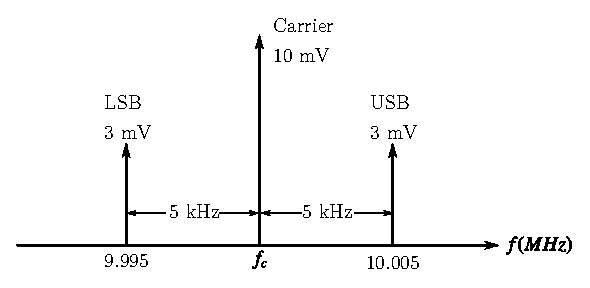
\includegraphics{chap8/fig8.5.eps}

\smallskip
{\bf Fig.~P8.5}
\end{figure}
\end{solution}

\eject

\begin{problem}\label{prob8.6}
A sinusoidal carrier voltage of frequency 1200 kHz is amplitude
modulated by a sinusoidal voltage of frequency 20 kHz resulting in
maximum and minimum modulated carrier amplitude of 110 V and 90 V
respectively. Calculate
\begin{itemize}
\item[(i)] the frequency of lower and upper sidebands 
\item[(ii)] the unmodulated carrier amplitude
\item[(iii)] modulation index
\item[(iv)] amplitude of each sideband
\end{itemize}
\end{problem}

\begin{solution}
Given $\rmf_\rmc = 1200$ kHz, ~ $\rmf_\rmm = 20$ kHz
$$
\rmE_{\text{ cmax}} = 110 \rmV, ~~ \rmE_{\text{ cmin}} = 90 \rmV
$$
\begin{itemize}
\item[(i)] Lower sideband frequency = $\rmf_\rmc - \rmf_\rmm =
(1200-20)$ kHz

\smallskip
\hspace{4.1cm} = 1180 kHz

\smallskip
Upper sideband frequency = $\rmf_\rmc +\rmf_\rmm = (1200+20)$ kHz

\smallskip
\hspace{4.1cm} = 1220 kHz

\item[(ii)] Unmodulated carrier amplitude ~$\rmE_\rmc = \dfrac{\rmE_{\text{ cmax}} +
\rmE_{\text{ cmin}}}{2}$

\smallskip
\hspace{5.4cm} = $\dfrac{110+90}{2}$

\smallskip
\hspace{5.4cm} = 100 V

\smallskip
\item[(iii)] Modulation index ~ $\rmm = \dfrac{\rmE_{\text{ cmax}} - \rmE_{\text{
cmin}}}{\rmE_{\text{ cmax}} + \rmE_{\text{ cmin}}}$

\smallskip
\hspace{3.38cm} = $\dfrac{110-90}{110+90}$

\smallskip
\hspace{3.38cm} = 0.1

\smallskip
\item[(iv)] Amplitude of each sideband = $\dfrac{\rmm \rmE_\rmc}{2}$

\smallskip
\hspace{4.35cm} = $\dfrac{0.1 \times 100}{2}$

\smallskip
\hspace{4.35cm} = 5 V
\end{itemize}
\end{solution}

\eject

\begin{problem}\label{prob8.7}
A sinusoidal voltage amplitude modulates another sinusoidal voltage of
amplitude 2 kV results in two sideband terms each of amplitude 200
V. Calculate the modulation index.
\end{problem}

\begin{solution}
Given $\rmE_\rmc  = 2$ kV, \; $\dfrac{\rmm \,\rmE_\rmc}{2} = 200$ V
$$
\therefore ~ \rmm = \frac{2 \times 200}{\rmE_\rmc} = \frac{2 \times 200}{2 \times 10^3} = 0.2
$$
\end{solution}

\begin{problem}\label{prob8.8}
The rms value of an RF carrier voltage is 100 V. After amplitude
modulation by a sinusoidal audio voltage, the rms value of the carrier
voltage increases to 108 V. Calculate the modulation index.
\end{problem}

\begin{solution}
Given ~$\rmE_{\text{ carr}} = 100$ V, ~$\rmE_{\rmt,\text{rms}}$ = 108 V

\smallskip
We have ~$\rmP_\rmt = \rmP_\rmc \left(1 + \dfrac{\rmm^2}{2} \right)$
\begin{align*}
\frac{\rmE^2_{\rmt,\text{rms}}}{\rmR} & = \frac{\rmE^2_{\text{
carr}}}{\rmR} \left(1 + \frac{\rmm^2}{2} \right)\\[4pt]
\therefore ~ \rmE^2_{\rmt,\text{rms}} & =
\rmE^2_{\text{ carr}} \left(1+\frac{\rmm^2}{2} \right)\\[4pt]
108^2 & = 100^2 \left(1+\frac{\rmm^2}{2} \right)
\end{align*}
$\therefore$ ~ Modulation index  $\rmm = 0.577$.
\end{solution}

\begin{problem}\label{prob8.9}
A broadcast transmitter radiates 4.9 kW, when the modulation
percentage is 60. Calculate the total power when the modulation has
been reduced to 40\%.
\end{problem}

\begin{solution}
Given ~$\rmP_\rmt = 4.9$ kW ~when~ $\rmm=60\%$ ~i.e.,~ $\rmm=0.6$

\medskip
\begin{tabbing}
We have, total power ~~$\rmP_\rmt$ \= = \= $\rmP_\rmc \left(1+\dfrac{\rmm^2}{2} \right) $\\[0.2cm]
\hspace{1.15cm} Carrier power $\rmP_\rmc$ \> = \> $\dfrac{\rmP_\rmt}{1 + \frac{\rmm^2}{2}}$\\[0.2cm]
\> = \> $\dfrac{4.9 \times 10^3}{1+\frac{0.6^2}{2}}$\\[0.2cm]
\hspace{3.4cm} $\rmP_\rmc$ \> = \> 4.15 kW
\end{tabbing}
$\therefore$ When $\rmm=40$\%, i.e.,  $\rmm=0.4$ ~the total power ~$\rmP_\rmt
=\rmP_\rmc  \left(1+\dfrac{\rmm^2}{2} \right)$
$$ 
\therefore ~ \rmP_\rmt = 4.15 \times 10^3 \left(1+\dfrac{0.4^2}{2} \right) =
4.48 ~\rmk\rmW \hspace{2cm}
$$
\end{solution}

\begin{problem}\label{prob8.10}
A radio transmitter using amplitude modulation has unmodulated
carrier power output of 10 kW and can be modulated to a maximum depth
of 80\%  by a sinusoidal modulating wave (a) Find power of the
modulated wave. (b) Find the value to which the unmodulated carrier
power may be increased, if the maximum permitted modulation is 50\%.
\end{problem}

\begin{solution}
Given: 
\begin{itemize}
\item[(a)] $\rmP_\rmc = 10$ kW ~ $\rmm=80\% = 0.8$
\begin{tabbing}
$\therefore $~ Power in the modulated wave $\rmP_\rmt$
\= = \= $\rmP_\rmc \left(1+\dfrac{\rmm^2}{2} \right)$\\[4pt]
\> = \> $10 \times 10^3 \left(1+ \dfrac{0.8^2}{2} \right)$\\
\> = \> 13.2 \rmk\rmW.
\end{tabbing}

\item[(b)] 13.2 kW is the maximum power which may be handled by the
transmitter. The increased unmodulated carrier power is give 
\begin{align*}
13.2 \times 10^3 & = \rmP_\rmc \left(1+\dfrac{0.5^2}{2} \right)\\
\therefore  ~\rmP_\rmc & = 11.73 ~\rmk\rmW
\end{align*}
\end{itemize}
\end{solution}

\begin{problem}\label{prob8.11}
A 100 V, 100 kHz carrier wave is modulated by a 10 V, 1 kHz signal to
the depth of 50\%. Write the AM wave equation.
\end{problem}

\begin{solution}
Given: $\rmE_\rmc = 100$ V; ~$\rmf_\rmc = 100$ kHz, ~$\rmE_\rmm = 10$ V, ~$\rmf_\rmm = 1$ kHz;
~$\rmm=50\% = 0.5$
\begin{align*}
\therefore ~ \omega_\rmm & = 2 \pi \rmf_\rmm = 2 \pi \times 1 \times 10^3 =
2 \times 10^3 \pi \text{ ~rad/sec }\\
\&~~ \omega_\rmc & = 2 \pi \rmf_\rmc = 2 \pi \times 100 \times 10^3 = 2 \times
10^5 \text{ ~rad/sec~ } \& ~\rmm = \frac{\rmE_\rmm}{\rmE_\rmc} = \frac{10}{100} = 0.1
\end{align*}
AM wave equation is given by,
\begin{align*}
\rme(\rmt) & = \rmE_\rmc  (1+\rmm \sin \omega_\rmm \rmt) \sin \omega_\rmc \rmt\\
& = 100 (1 + 0.1 \sin 2 \times 10^3 \pi \rmt) \sin 2 \times 10^5 \pi \rmt
\end{align*}
\end{solution}

\begin{problem}\label{prob8.12}
An AM wave is represented by the equation 
$$ 
\rme(\rmt) = 20 (1+0.7 \sin 6280 ~\rmt) \sin 628000 ~\rmt.
$$
Determine: (i) modulation index (ii) carrier amplitude (iii) carrier
frequency (iv) signal frequency (v) signal amplitude  (vi) maximum
amplitude of AM wave (vii) minimum amplitude of AM wave (viii) bandwidth.
\end{problem}

\begin{solution}
Given: $\rme(\rmt) = 20 (1+0.7 \sin 6280~\rmt) \sin 62800 ~\rmt$

Comparing with AM wave equation
$$
\rme(\rmt) = \rmE_\rmc (1+\rmm \sin \omega_\rmm \rmt) \sin \omega_\rmc \rmt.
$$
we have ~~$\rmE_\rmc = 20$ V; ~$\rmm=0.7$; ~$\omega_\rmm=6280$ rad/sec;~
 $\omega_\rmc = 62800$ rad/sec.

\smallskip
 $\rmm = \dfrac{\rmE_\rmm}{\rmE_\rmc}\qquad ~\therefore  \rmE_\rmm = \rmm \rmE_\rmc =
0.7 \times 20= 14$ V.
\begin{align*}
\omega_\rmm & = 2 \pi \rmf_\rmm = 6280 \text{ rad/sec} \qquad \therefore ~\rmf_\rmm = 1
\text{ kHz}.\\
\omega_\rmc & = 2 \pi \rmf_\rmc = 62800 \text{
rad/sec} \qquad \therefore ~\rmf_\rmc = 10 \text{ kHz}.
\end{align*}

$\rmE_{\text{ cmax}} = \rmE_\rmc + \rmE_\rmm = \rmE_\rmc + \rmm \rmE_\rmc = 20 + 14 = 34 $ V 

\smallskip
$\rmE_{\text{ cmin}} = \rmE_\rmc - \rmE_\rmm = \rmE_\rmc - \rmm \rmE_\rmc = 20 - 14 = 6$ V.

\smallskip
Band width = $2 \omega_\rmm = 12560$ rad/sec

\hspace{1.8cm} = $2 \rmf_\rmm = 2$ kHz.
\end{solution}

\begin{problem}\label{prob8.13}
Unmodulated RF carrier power of 2 kW sends a current of 5A rms through
an antenna. On amplitude modulation by another sinusoidal voltage, the
antenna current increases to 5.9A. Calculate (i) the modulation index
(ii) carrier power after modulation.
\end{problem}

\begin{solution}
Given ~$\rmI_\rmt = 5.9$ A, ~$\rmI_\rmc = 5$ A, ~$\rmP_\rmc = 2$ kW

\medskip
We have $\rmI_\rmt = \rmI_\rmc \sqrt{1+\dfrac{\rmm^2}{2}}$

\smallskip
\hspace{1.1cm} $5.9 = 5 \times \sqrt{1+\dfrac{\rmm^2}{2}}$
\begin{itemize}
\item[(i)] $\therefore$ Modulation index $\rmm = 0.885$

\item[(ii)] Carrier power after modulation ~ $\rmP_\rmt =
\rmP_\rmc \left(1+ \dfrac{\rmm^2}{2} \right)$

\hspace{5.4cm} = $2 \times 10^3 \left(1+ \dfrac{0.885^2}{2} \right)$

\hspace{5cm} $\rmP_\rmt$ = 2.78 kW
\end{itemize}
\end{solution}

\begin{problem}\label{prob8.14}
The antenna current of an AM transmitter is 8A, when only the carrier
is sent, but it increases to 8.93 A, when the carrier is modulated by
a single sinewave. Find the\break percentage modulation. Determine the
antenna current when the depth of modulation changes to 0.8.
\end{problem}

\begin{solution}
Given ~$\rmI_\rmc = 8$ A, ~$\rmI_\rmt =8.93$ A

\medskip
We have $\rmI_\rmt = \rmI_\rmc \sqrt{1+\dfrac{\rmm^2}{2}}$

\medskip
\hspace{0.9cm} $8.93 = 8\times \sqrt{1+\dfrac{\rmm^2}{2}}$

\smallskip
$\therefore$ ~Modulation index : $\rmm = 0.701 = 70.1 \%$

When $\rmm = 0.8$,
\begin{tabbing}
Antenna current ~$\rmI_\rmt$ \= =  \= $\rmI_\rmc \sqrt{1+\dfrac{\rmm^2}{2}}$\\[0.1cm]
\> = \> $8 \times \sqrt{1+\dfrac{0.8^2}{2}}$\\[4pt]
\hspace{2.6cm} $\rmI_\rmt$ \> = \> 9.19 A
\end{tabbing}
\end{solution}

\begin{problem}\label{prob8.15}
An AM transmitter radiates 9 kW with the carrier unmodulated and
10.125 kW, when the carrier is sinusoidally modulated. Calculate the
modulation index. If another sinewave corresponding to 40\% modulation
is transmitted simultaneously, determine the total radiated power.
\end{problem}

\begin{solution}
Given ~~$\rmP_\rmc = 9 $ kW, ~~$\rmP_\rmt = 10.125$ kW
\begin{tabbing}
We have ~$\rmP_\rmt$ \= = \= $\rmP_\rmc \left(1+\dfrac{\rmm^2}{2} \right)$\\[4pt]
\hspace{0.6cm} 10.125 \> = \> $9 \left(1+\dfrac{\rmm^2}{2} \right)$\\[4pt]
\hspace{1.4cm} $\rmm$ \> = \> $\rmm_1 = 0.5$
\end{tabbing}

If another sinewave is transmitted simultaneously with modulation
depth $\rmm_2 = 40$\%, i.e., $\rmm_2 = 0.4$, then the total modulation
index,
\begin{align*}
\rmm & = \sqrt{\rmm^2_1 + \rmm^2_2}\\
& = \sqrt{0.5^2 +0.4^2}\\
\rmm & = 0.64
\end{align*}
\begin{tabbing}
$\therefore$ Total radiated power ~ $\rmP_\rmt$ \= = \=
$\rmP_\rmc \left(1+\dfrac{\rmm^2}{2} \right) $\\[4pt]
\> = \> $9 \times 10^3 \times \left(1+\dfrac{0.64^2}{2} \right)$\\
\hspace{3.7cm} $\rmP_\rmt$ \> = \> 10.84 kW
\end{tabbing}
\end{solution}

\begin{problem}\label{prob8.16}
The antenna current of an AM broadcast transmitter, modulated to a
depth of 40\% by an audio sinewave is 11 A. It increases to 12 A as a
result of simultaneous modulation by another audio sinewave. What is
the modulation index due to this second wave?
\end{problem}

\begin{solution}
Given ~$\rmm_1 = 40\%$, ~$\rmI_\rmt = 11$ A
\begin{tabbing}
We have ~ $\rmI_\rmt$ \= = \= $\rmI_\rmc \sqrt{1+\dfrac{\rmm^2_1}{2}}$\\[4pt]
\hspace{1.4cm} 11 \> = \> $\rmI_\rmc \sqrt{1+\dfrac{0.4^2}{2}}$\\[4pt]  
\hspace{1cm} $\therefore$ ~ $\rmI_\rmc$ \> = \> 10.58 A
\end{tabbing}

In the second case, it becomes 12 A, as a result of simultaneous
modulation by another sinewave. Let the total modulation index be $\rmm$.
\begin{align*}
\rmI_\rmt & = \rmI_\rmc \sqrt{1 + \dfrac{\rmm^2}{2}}\\
\therefore ~ 12 & = 10.58 \times \sqrt{1+\frac{\rmm^2}{2}}
\end{align*}
$\therefore $~ Total modulation index ~$\rmm = 0.757$

\smallskip
We have ~$\rmm = \sqrt{\rmm^2_1 + \rmm^2_2}$

\smallskip
Modulation index due to the second wave,
\begin{align*}
\rmm_2 & = \sqrt{\rmm^2 -\rmm^2_1}\\[4pt]
& = \sqrt{0.757^2 -0.4^2}\\[4pt]
\rmm_2 & = 0.643
\end{align*}
\end{solution}

\eject

\begin{problem}\label{prob8.17}
An audio signal given by $15 \sin 2\pi ~(2000)\rmt$ amplitude
modulates a sinusoidal carrier wave $60 \sin
2 \pi~(100,000)\rmt$. Determine (i) modulation index (ii) frequencies of
signal and carrier (iii) frequency components of the modulated wave. 
\end{problem}

\begin{solution}
Given Modulating signal $\rme_\rmm(\rmt) = \rmE_\rmm \sin \omega_\rmm \rmt = 15 \sin 2 \pi
(2000) \rmt$
\begin{align*}
& \therefore \rmE_\rmm = 15 V, ~\rmf_\rmm = 2000 ~\text{ Hz} = 2 ~\text{ kHz}.\\
& \text{Carrier signal } \rme_\rmc (\rmt) = \rmE_\rmc \sin \omega_\rmc \rmt = 60 \sin
2 \pi~(100,000)\rmt\\
& \therefore \rmE_\rmc = 60\rmV,  ~\rmf_\rmc = 100,000 \text{ Hz} =
100 \text{ kHz}.
\end{align*}
\begin{itemize}
\item[(i)] Modulation index ~ $\rmm = \dfrac{\rmE_\rmm}{\rmE_\rmc} = \dfrac{15}{60} =
0.25$

\item[(ii)] Frequency of the signal $\rmf_\rmm = 2$ kHz

Frequency of the carrier $\rmf_\rmc = 100$ kHz

\item[(iii)] The 3 frequency components of the modulated carrier wave
are, 
$$
\rmf_\rmc = 100 \text{ kHz }, ~~\text{USB : } \rmf_\rmc+\rmf_\rmm =
102 \text{ kHz}, ~~\text{LSB : } \rmf_\rmc - \rmf_\rmm = 98 \text{ kHz}
$$
\end{itemize}
\end{solution}

\begin{problem}\label{prob8.18}
A bandwidth of 15 MHz is available for AM transmission. If the maximum
audio signal frequency used for modulating the carrier is not to
exceed 15 kHz, how many stations can broadcast within this band
simultaneously without interfering with each other ?
\end{problem}

\begin{solution}
Bandwidth required by each station $= 2 \rmf_{\rmm(\text{ max})} = 2 \times
15 $kHz

\hspace{8.3cm} = 30 kHz

$\therefore$~ the number of stations that can broadcast within this
frequency band of 15 MHz \break is $=\dfrac{15~\text{MHz}}{30 ~\text{kHz}} = 500$.
\end{solution}

\section{Limitations of Amplitude modulation}\label{sec8.6}
The limitations of amplitude modulation are 
\begin{itemize}
\item[(i)] In AM, the  useful power (message) is contained in the
sidebands. Even at 100\% modulation ($m=1$), the sideband contains
only 33\%  of the total power (i.e., $\rmP_\rmt =1.33 \rmP_\rmc$) and
hence the modulation efficiency is poor.

\item[(ii)] The transmitters employing amplitude modulation has very
poor range.

\item[(iii)] The reception of the amplitude signal is very noisy,
i.e., the receiver picks up all the surrounding noise along with the signal.
\end{itemize}

\section{AM Detection (Demodulation)}\label{sec8.7}
The process of detecting (seperating) the original modulating
(message) signal from the modulated signal is called detection or
demodulation. To recover the message signal from the AM signal at the
receiving end, the envelop of AM signal has to be detected. This is
acheived by passing the AM signal through a diode to cut-off the lower
half and the peaks are detected and smoothened by a parallel RC
circuit as shown in Fig.~\ref{fig8.7} Assuming the diode is ideal, the output
voltage $\rme_\rmo(\rmt)$ is always the capacitor voltage.
\setcounter{figure}{6}
\begin{figure}[H]
\centering
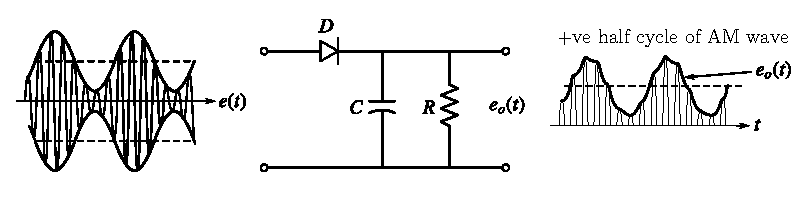
\includegraphics{chap8/fig8.7.eps}
\caption{Demodulation process}\label{fig8.7}
\end{figure}

When e(t) rises to the first peak, the capacitor charges to the peak
value. As e(t) goes above plate, the diode conducts and capacitor
starts charging to the next peak and e(t) increases. Similarly, as
e(t) falls below peak, the diode stops conducting and capacitor
stops charging and discharges through R and e(t) decreased. This
process repeats and $\rmv_0(\rmt)$ resembles the message signal. The
resemblense is better if the time constant RC meet the condition
\begin{align*}
\rmR\rmC >> \rmT_\rmc &= \frac{1}{\rmf_\rmc} = \frac{\omega_\rmc}{2\Pi} ;\quad \rmT_\rmc = \text{
carrier time period. } \\
\rmR\rmC << \rmT_\rmm & =  \frac{1}{\rmf_\rmm} = \frac{\rmw_\rmm}{2\pi} ; \quad \rmT_\rmm = \text{
time period of message signal } \\
\therefore \hspace{1cm} \frac{\omega_\rmc}{2\pi}
& \leq \rmR\rmC \leq \frac{\omega_\rmm}{2\pi}  \hspace{1cm}
\end{align*}

The AM wave is given 
\begin{equation*}
\rme(\rmt)= \rmE_\rmc (1+\rmm \sin \omega_\rmn \rmt) \sin \omega_\rmc \rmt 
\end{equation*}

Therefore the detected envelop (capacitor voltage) is 
\begin{equation*}
\rme_\rmm (\rmt) = \rmE_\rmc (1+\rmE_\rmc \sin \omega_\rmm \rmt) 
\end{equation*}
Eqn.~\eqref{???} indicates that the detected envelop suffers from the
disadvantage that it contains DC components $\rmE_\rmc$ and also ripples
which are unwanted. There can be filtered out by a simple RC lowpass circuit.

\section{Frequency Modulation FM}\label{label8.8}

\textit{Frequency modulation FM} is a process in which the frequency
of the carrier signal is varied in accordance with the instantaneous
amplitude of the modulating signal. In FM. amplitude of the carrier
voltage does not change. The amount  of change in frequency is
determined by the amplitude of the modulating signal whereas the rate
of frequency change is determined by the frequency of the modulating
signal. Fig.~\ref{fig8.8}(a) shows a modulating signal $\rme_\rmm(\rmt)$,
Fig.~\ref{fig8.8}(b) shows a carrier wave $\rme_\rmc(\rmt)$ and
Fig.~\ref{fig8.8}(c) shows frequency modulated signal e(t).
\begin{figure}[H]
\centering
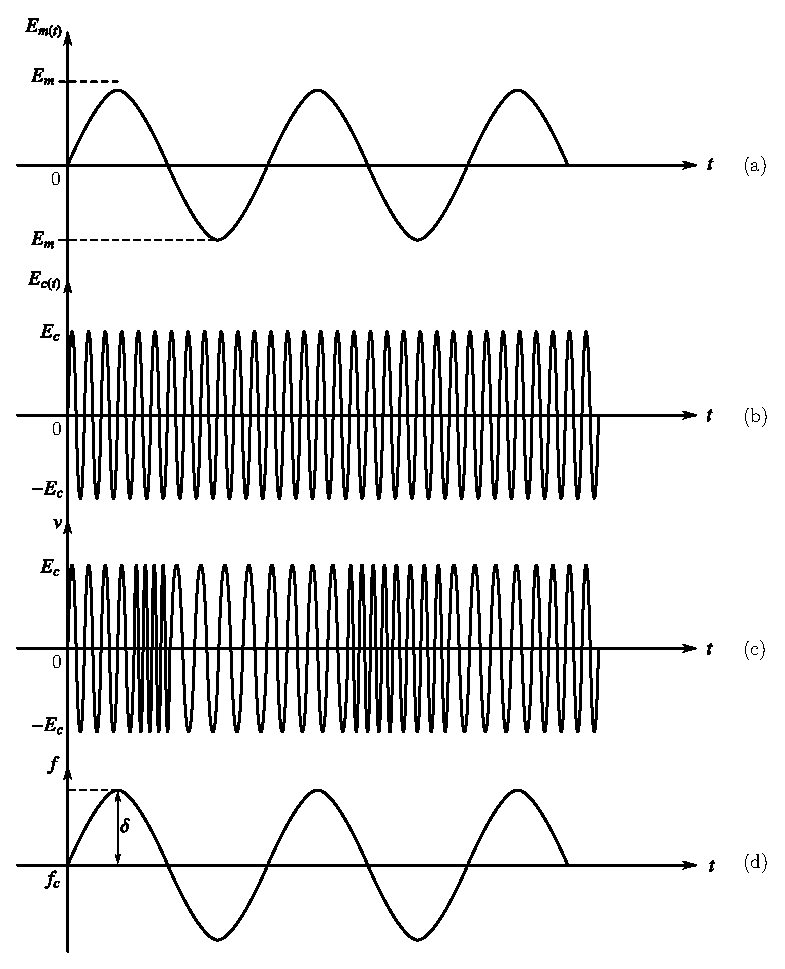
\includegraphics[scale=0.83]{chap8/fig8.6.eps}
\caption{Different waveforms of FM signal (a) modulating signal (b)
carrier wave (c) FM signal (d) f Vs t.}\label{fig8.8}
\end{figure}

Fig.~\ref{fig8.8}(d) shows the instantaneous frequency of the
frequency modulated wave with respect to time. Observe that the
frequency variation with respect to time is identical to the shape of
the modulating signal $\rme_\rmm(\rmt)$.


\heading{\textit{Expression for frequency modulated voltage:}}

Let the sinusoidal modulating signal be given by,
\begin{equation}
\rme_\rmm(\rmt) = \rmE_\rmm \cos \omega_\rmm \rmt\label{eq8.24}
\end{equation}
where $\omega_\rmm$ = angular frequency of the modulating signal (rad/sec)

\quad~$\rmV_\rmm$ = amplitude of the modulating signal (V)

Let the carrier voltage be given by, 
\begin{equation}
\rme_\rmc(\rmt) = \rmE_\rmc \sin (\omega_\rmc \rmt + \phi_\rmc) \label{eq8.25}
\end{equation}
where $\omega_c$ = angular frequency of the carrier signal (rad/sec)

\quad~$\rmE_\rmc$ = amplitude of carrier wave (V)

\noindent
\quad~and $\phi_\rmc$ = phase angle (rad)

Let 
\begin{equation}
\theta = \omega_\rmc \rmt  + \phi_\rmc\label{eq8.26}
\end{equation}

In Eqn.~\eqref{eq8.26}, $\theta$ is the total instantaneous phase
angle of the carrier wave. Therefore Eqn.\eqref{eq8.25} can be written
as 
\begin{equation}
\rme_\rmc (\rmt) = \rmE_\rmc \sin \theta \label{eq8.27}
\end{equation}

Thus, the angular frequency $\omega_\rmc$ of the carrier wave is related
to $\theta$ as given by 
\begin{equation}
\omega_\rmc = \dfrac{\rmd  \theta}{\rmd\rmt} \label{eq8.28}
\end{equation}

On frequency modulation, the frequency of the carrier wave no longer
remains constant but  varies with time in accordance with the
instantaneous amplitude of the modulating voltage.

From Fig.~\ref{fig8.8}(d), it is seen that the instantaneous frequency
of the frequency modulated wave is give by
\begin{equation}
\rmf = \rmf_\rmc (1+\rmk \rme_\rmm (\rmt)) \label{eq8.29}
\end{equation}

Substituting Eqn.~\eqref{eq8.24} in Eqn.~\eqref{eq8.29},
\begin{equation}
\rmf= \rmf_\rmc (1+\rmk \rmE_\rmm \cos \omega_\rmm \rmt)\label{eq8.30}
\end{equation}
where~ $\rmf_\rmc$ = frequency of unmodulated carrier wave.

~\quad ~k = constant of proportionality.

$\rme_\rmm$(t) = $\rme_\rmm \cos \omega_\rmm \rmt$ = instantaneous amplitude of modulating signal.

~~~$\rmE_\rmm$ = Maximum amplitude of modulating signal.

The maximum deviation of frequency in the modulated carrier wave will
occur when the cosine term in Eqn.~\eqref{eq8.30} has its maximum
value. i.e., $\pm 1$. Under this condition, the instantaneous
frequency will be
\begin{align}
\rmf & = \rmf_\rmc (1 +\rmk \rmE_\rmm)\label{eq8.31}\\
\rmf & = \rmf_\rmc + \rmk \rmE_\rmm \rmf_\rmc \label{eq8.32}
\end{align}

Thus, the maximum deviation of frequency is given by 
\begin{equation}
\delta = \rmk \rmE_\rmm \rmf_\rmc \label{eq8.33}
\end{equation}

It is shown in Fig.~\ref{fig8.8}(d)

From Eqn.~\eqref{eq8.30}, we have
\begin{equation}
\omega = \omega_\rmc (1 + \rmk \rmE_\rmm \cos \omega_\rmm \rmt)\label{eq8.34}
\end{equation}

In order to find the phase angle $\theta$, $\omega$ must be integrated
with respect to time t. Thus integrating Eqn.~\eqref{eq8.28},
\begin{align}
\phi & = \int \omega \rmd\rmt\notag\\
& = \int \omega_\rmc (1+ \rmk \rmE_\rmm \cos \omega_\rmm \rmt) \rmd\rmt\notag\\
& = \omega_\rmc \int (1 + \rmk \rmE_\rmm \cos \omega_\rmm \rmt) \rmd\rmt\notag\\
& = \omega_\rmc \left[\rmt + \frac{\rmk \rmE_\rmm \sin \omega_\rmm
t}{\omega_\rmm} \right]\notag\\
& = \omega_\rmc \rmt + \frac{\rmk \rmE_\rmm \omega_\rmc}{\omega_\rmm} \sin \omega_\rmm \rmt \notag\\
\phi & = \omega_\rmc \rmt
+ \frac{\rmk \rmE_\rmm \rmf_\rmc}{\rmf_\rmm} \sin \omega_\rmm \rmt\label{eq8.35}
\end{align}

Substituting Eqn.~\eqref{eq8.33} in Eqn.~\eqref{eq8.35}, 
\begin{equation}
\theta = \omega_\rmc \rmt + \frac{\delta}{\rmf_\rmm} \sin \omega_\rmm \rmt\label{eq8.36}
\end{equation}

Substituting Eqn.~\eqref{eq8.36} in Eqn.~\eqref{eq8.27}, we get the
expression for frequency modulated wave as
\begin{equation}
\rme(\rmt) = \rmE_\rmc \sin (\omega_\rmc \rmt + \frac{\delta}{\rmf_\rmm} \sin \omega_\rmc \rmt)\label{eq8.37}
\end{equation}

The modulation index $\rmm_\rmf$ for FM is defined as,
\begin{equation}
\rmm_\rmf = \frac{\text{maximum frequency deviation}}{\text{modulating
frequency}} = \frac{\delta}{\rmf_\rmm}\label{eq8.38}
\end{equation}

Substituting Eqn.~\eqref{eq8.38} in Eqn.~\eqref{eq8.37},
\begin{equation}
\rme = \rmE_\rmc \sin (\omega_\rmc \rmt
+ \rmm_\rmf \sin \omega_\rmm \rmt)\label{eq8.39}
\end{equation}
Eqn.~\eqref{eq8.39} is known as the expression  for the FM wave.

\heading{\textit{Bandwidth required for FM wave}}

Theoritically, the bandwidth required for the transmission of FM wave
is infinite. But as a good approximation, Carson's rule (thumb rule)
states that the bandwidth required to pass an FM wave is twice the sum
of the deviation and the highest modulating frequency. This
approximation give a fairly accurate result, if the modulation index
is greater than 6.
\begin{equation}
\text{Band width } \simeq 2(\delta + \rmf_\rmm)\label{eq8.40}
\end{equation}


\begin{center}
\rule{4cm}{1pt}\\
{\bf\Large Problems}\\[-3pt]
\rule{4cm}{1pt}
\end{center}

\begin{problem}\label{prob8.19}
What is the modulation index of an FM carrier having a carrier swing
of 120 kHz and a modulating signal of 10 kHz.
\end{problem}

\begin{solution}
Given $\rmf_\rmm =  10$ kHz.

\smallskip
We know that, carrier swing = $2 \times$ frequency deviation = 120 kHz

\smallskip
$\therefore$ Frequency deviation $\delta = 120 \times 10^3 = 60$ kHz

\smallskip
$\therefore$ Modulation index $\rmm_\rmf = \dfrac{\delta}{\rmf_\rmm}
= \dfrac{60 \times 10^3}{10 \times 10^3} = 6$
\end{solution}

\begin{problem}\label{prob8.20}
An FM signal has a resting frequency of 100 MHz and the highest
frequency of 100.05 MHz when modulated by an audio signal of 5
kHz. Determine (i) frequency deviation (ii) carrier swing (iii)
modulation index.
\end{problem}

\eject

\begin{solution}
Given $\rmf_\rmc = 100$ MHz, ~~$\rmf_\rmh = 100.5$ MHz

\hspace{1.9cm} $\rmf_\rmm$ = 5 kHz
\begin{itemize}
\item[(i)] Frequency deviation $\delta = \rmf_\rmh - \rmf_\rmc = (100.05-100)$MHz
= 50 kHz

\item[(ii)] Carrier swing $= 2 \delta = 2 \times 50$ kHz = 100 kHz

\item[(iii)] Modulation index = $\rmm_\rmf = \dfrac{\delta}{\rmf_\rmm} = \dfrac{50
\text{ kHz}}{5 \text{ kHz}} = 10$
\end{itemize}
\end{solution}

\begin{problem}\label{prob8.21}
An FM signal has resting frequency of 105 MHz and highest frequency of
105.03 MHz when modulated by a signal of frequency 5 kHz. Determine
(i) frequency deviation (ii) carrier swing (iii) modulation index (iv)
lowest frequency of the FM wave.
\end{problem}

\begin{solution}
Given $\rmf_\rmc = 105$ MHz, $\rmf_\rmh = 105.03$ MHz, $\rmf_\rmm = 5$
kHz.
\begin{itemize}
\item[(i)] Frequency deviation $\delta = \rmf_\rmh - \rmf_\rmc = (100.03 -
100)$MHz = 30 kHz.

\item[(ii)] Carrier swing = $2 \delta = 2 \times 30$ kHz = 60 kHz

\item[(iii)] Modulation index = $\rmm_\rmf = \dfrac{\delta}{\rmf_\rmm} = \dfrac{30
\times 10^3}{5 \times 10^3} = 6$

\item[(iv)] Lowest frequency of the FM wave = $\rmf_\rmc - \delta = 105$ MHz
- 30 kHz

\hspace{5.3cm} = 104.97 MHz
\end{itemize}
\end{solution}

\begin{problem}\label{prob8.22}
A 10 kHz audio signal is used to frequency modulate a 100 MHz carrier
causing a frequency deviation of 80 kHz. Determine (i) modulation
index (ii) bandwidth of FM signal.
\end{problem}

\begin{solution}
Given ~$\rmf_\rmc = 100$ MHz, ~$\rmf_\rmm = 10$ kHz, ~$\delta =80$ kHz
\begin{itemize}
\item[(i)] Modulation index $\rmm_\rmf
= \dfrac{\delta}{\rmf_\rmm}= \dfrac{80 \text{kHz}}{10\text{ kHz}}=8$

\item[(ii)] According to Carson's rule, bandwidth ~$\simeq 2 (\delta + \rmf_\rmm)$

\hspace{6.1cm} = 2 (80 +10)kHz

\hspace{6.1cm} = 180 kHz
\end{itemize}
\end{solution}

\begin{problem}\label{8.20}
Find the carrier and modulating frequencies, the modulation index and
the maximum deviation of the FM wave represented by the voltage
equation $\rme(\rmt) = 10 \sin (6 \times 10^8 \rmt + 7 \sin 1250 \rmt)$.
\end{problem}

\begin{solution}
Comparing the equation with Eqn.~\eqref{eq8.39}, we get,
\begin{align*}
\rme_\rmc & = 10 \rmV, ~\omega_\rmc = 2 \pi \rmf_\rmc = 6 \times
10^8 \text{ rad/sec }  \quad \therefore ~ \rmf_\rmc = 95.5 ~\text{
MHz} \\
\omega_\rmm & = 2\pi \rmf_\rmm = 1250 \text{ rad/sec } \qquad \therefore \rmf_\rmm = 199 ~\rmH\rmz
\end{align*}

Modulation index $\rmm_\rmf =7$

\smallskip
We have $\rmm_\rmf = \dfrac{\delta}{\rmf_\rmm}$

\smallskip
$\therefore$ Maximum deviation $\delta$ = $\rmm_\rmf \times \rmf_\rmm$

\hspace{3.75cm} = $7 \times 199 = 1393$ Hz
\end{solution}

\begin{problem}\label{prob8.23}
In an FM modulator, when the modulating frequency is 600 MHz,
modulating voltage is 2.4 V and the modulation index is 1.5. What is
the modulation index when the frequency is reduced to 400 Hz and the
modulating voltage is simultaneously increased to 3.2 V.
\end{problem}

\begin{solution}
Given : $\rmf_\rmm = 600$ Hz, ~$\rmm_\rmf = 1.5$, ~$\rme_\rmm = 2.4$ V

\smallskip
We have $\rmm_\rmf = \dfrac{\delta}{\rmf_\rmm}$

\smallskip
$\therefore$ Frequency deviation $\delta = \rmm_\rmf \times \rmf_\rmm = 1.5 \times
600 = 900$ Hz

\smallskip
We know that the frequency deviation $\delta$ is proportional to
$\rmV_\rmm$. i.e., ~~$\delta \propto \rmV_\rmm$.

\smallskip
$\therefore \dfrac{\delta}{\rmE_\rmm}= \dfrac{900}{2.4} = 3.75 $  Hz/V

\smallskip
Now when $\rmE_\rmm = 3.2$,

\smallskip
$\delta = 375 \times 3.2 = 1200$ Hz

\smallskip
Then modulation index $\rmm_\rmf = \dfrac{\delta}{\rmf_\rmm}
= \dfrac{1200}{400} = 3$
\end{solution}

\begin{problem}\label{prob8.24}
When the modulating frequency in FM is 600 Hz and modulating voltage
is 3 V, the modulation index is 60. Calculate the maximum
deviation. What is the modulation index when the modulating frequency
is reduced to 400 Hz and the modulating voltage is simultaneously
raised to 4V.
\end{problem}

\begin{solution}
Given $\rmf_\rmm = 600$ Hz, ~$\rmE_\rmm = 3$ V, ~$\rmm_\rmf =60$

\smallskip
Maximum frequency deviation $\delta = \rmm_\rmf \rmf_\rmm= 60 \times 600 = 36$
kHz. We know that, the frequency deviation $\delta$ is proportional to
$\rmV_\rmm$. i.e., $\delta \propto \rmV_\rmm$.

\smallskip
$\therefore \dfrac{\delta}{\rmE_\rmm} = \dfrac{36~ \text{ kHz}}{3\rmV}
= 12$ kHz/V

\smallskip
Now when, $\rmE_\rmm = 4$ V
$$
\delta = 12 \times 10^3 \times 4 = 48 \text{ kHz}
$$

\smallskip
Then modulation index $\rmm_\rmf = \dfrac{\delta}{\rmf_\rmm} = \dfrac{48~\text{kHz}}{400} = 120$
\end{solution}

\section{Phase Modulation (PM)}\label{sec8.9}

It is a process in which the phase angle of a carrier voltage is
varied in accordance with the instantaneous value of the modulating
signal. The amplitude and frequency of the carrier voltage remains
unaltered after phase modulation.

\heading{\textit{Expression for phase modulated voltage :}}

\smallskip
Let the carrier voltage be
\begin{equation}
\rme_\rmc(\rmt) = \rmE_\rmc \sin (\omega_\rmc \rmt + \theta_\rmc)\label{eq8.41}
\end{equation}
and the modulating voltage be 
\begin{equation}
\rme_\rmm(\rmt) = \rmE_\rmm \sin \omega_\rmm \rmt \label{eq8.42}
\end{equation}
Instantaneous phase of the carrier before modulation is given by
\begin{equation}
\phi_\rmc (\rmt) = \theta + \rmk_\rmp \rme_\rmm(\rmt) \label{8.43}
\end{equation}
where kp is constant of proportionality.

Substituting Eqn.~\eqref{eq8.46} in \eqref{eq8.47},
\begin{equation}
\phi(\rmt) = \omega_\rmc \rmt + \theta_\rmc + \rmk_\rmp \rme_\rmm(\rmt)\label{eq8.44}
\end{equation}

Substituting Eqn.~\eqref{eq8.45} in \eqref{eq8.48}, we get,
\begin{equation}
\phi(\rmt) = \omega_\rmc \rmt + \theta_\rmc + \rmk_\rmp \rmE_\rmm \sin \omega_\rmm \rmt\label{eq8.45}
\end{equation}

The phase modulated carrier voltage is then obtained from
Eqn.~\eqref{eq8.44} as, 
\begin{equation}
\rme(\rmt) = \rmE_\rmc \sin (\omega_\rmc \rmt+ \theta_\rmc + \rmk_\rmp \rmE_\rmm \sin \omega_\rmm \rmt)\label{eq8.46}
\end{equation}

In PM, the constant phase angle $\theta$c has no role and can be
ignored. Then the expression for PM voltage becomes,
\begin{equation}
\rme(\rmt) = \rmE_\rmc \sin (\omega_\rmc \rmt + \rmk_\rmp \rmE_\rmm \sin \omega_\rmm \rmt)\label{eq8.47}
\end{equation}

Thus, the maximum phase deviation $\phi_\rmm = \rmk_\rmp \rmE_\rmm$

$therefore$ From Eqn.~\eqref{eq8.47}, we have,
\begin{align}
\rme(\rmt) & = \rmE_\rmc \sin (\omega_\rmc \rmt+ \phi_\rmm \sin \omega_\rmm \rmt) \label{eq8.48}\\
\rme(\rmt) & = \rmE_\rmc \sin (\omega_\rmc \rmt + \rmm_\rmp \sin \omega_\rmm \rmt)\label{eq8.49}
\end{align}
where $\rmm_\rmp= \phi_\rmm$ is the modulation index for PM.

One important point to noted in PM is that the modulation index $\rmm_\rmp =
\phi_\rmm$ is independent of modulating frequency $\rmf_\rmm$, whereas in FM
the modulation index $\rmm_\rmf$ is inversely proportional to the
modulating frequency $\rmf_\rmm$. Hence in PM. for all values of modulating
frequency $\rmf_\rmm$, the phase deviation $\phi_\rmm$ remains constant.

The PM as such not used in any practical transmission systems, but it
is possible to obtain FM from PM by using Armstrong system.

\begin{center}
\rule{4cm}{1pt}\\
{\bf\Large Problems}\\[-3pt]
\rule{4cm}{1pt}
\end{center}

\begin{problem}\label{prob8.25}
A 25 MHz carrier is modulated by a 400 Hz audio sine wave. If the
carrier voltage is 4V, maximum deviation is 10 kHz, and same
modulation index for both FM and PM, write the equation of this
modulate wave for,
(a) FM and (b) PM. If the modulating frequency is now changed to 2
kHz, all else remaining constant, write a new equation for (c) FM and
(d) PM.
\end{problem}

\begin{solution}
Given~ $\rmf_\rmc = 25$ kHz, ~$\rmf_\rmm = 400$ Hz\,,~ $\rmE_\rmc$ =
4V

\smallskip
Maximum deviation = $\delta = \phi_\rmm = 10$ kHz

\smallskip
$\therefore$ $\omega_\rmc = 2 \pi \rmf_\rmc = 2 \pi \times 25 \times 10^6 =
157\times 10^6$ rad/sec.

\smallskip
\quad$\omega_\rmc = 2 \pi \rmf_\rmm =  2 \pi \times 400 = 2513$ rad/sec.

\smallskip
$\therefore $ The modulation index $\rmm_\rmf = \rmm_\rmp = \phi_\rmm
= \dfrac{\delta}{\rmf_\rmm} = \dfrac{10000}{400} = 25$

\smallskip
$\therefore$ The expressions are
\begin{itemize}
\item[(a)] FM : $\rme(\rmt) = 4 \sin (157 \times 10^6 \rmt + 25 \sin
2513 \rmt)$

\item[(b)] PM : $\rme(\rmt) = 4 \sin (157 \times 10^6 \rmt + 25 \sin 2513 \rmt)$
\end{itemize}

When the modulating frequency is increased to 2 kHz,
$$
\omega_\rmm = 2 \pi \times 2 \times 10^3 = 12566 \text{ rad/sec.}
$$

\smallskip
Then modulation index in FM = $\rmm_\rmf = \dfrac{\delta}{\rmf_\rmm}= \dfrac{10000}{2000} = 5$

\smallskip
But in PM modulation index remains constant i.e., $\rmm_\rmp = 25$

\smallskip
$\therefore$ The expressions are
\begin{itemize}
\item[(c)] FM : e(t) = $4 \sin (157 \times 10^6 \rmt + 5 \sin 12566$~t)

\item[(d)] PM : e(t) = $4 \sin (157 \times 10^6 \rmt + 25 \sin 12566$~t)
\end{itemize}
\end{solution}

\vfill\eject

\begin{problem}\label{prob8.26}
A 20 MHz, 5V carrier is modulated by a 500 Hz sine wave. The maximum
frequency deviation is 15 kHz and the same modulation index is
obtained for both FM and PM. Write expressions for (a) FM and (b) PM.

\smallskip
If the modulating frequency is increased to 3 kHz, keeping other
things constant, write expressions for (c) FM and (d) PM.
\end{problem}

\begin{solution}
Given $\rmf_\rmc = 20$ MHz, $\rmE_\rmc = 5$V, $\rmf_\rmm = 500$ Hz

\smallskip
Maximum frequency deviation $= \delta = \phi_\rmm = 15$ kHz
\begin{align*}
\omega_\rmc & = 2 \pi \times 20 \times 10^6 = 125.7 \times 10^6 \text{
rad/sec}\\[4pt]
\omega_\rmm & = 2 \pi \times 500 = 3141.5 \text{ rad/sec}
\end{align*}

The modulation index $\rmm_\rmf = \rmm_\rmp = \varphi_\rmm = \dfrac{\delta}{\rmf_\rmm}
= \dfrac{15 \times 10^3}{500} = 30$

\smallskip
$\therefore$ ~ The expression are
\begin{itemize}
\item[(a)] FM : $\rme(\rmt) = 5 \sin (125.7 \times 106 \rmt + 30 \sin 3141.5 \rmt)$

\item[(b)] PM : $\rme(\rmt) = 5 \sin (125.7 \times 106 \rmt + 30 \sin 3141.5 \rmt)$
\end{itemize}

When the modulating frequency is increased to 3 kHz,
$$
\omega_\rmm = 2 \pi \rmf_\rmm = 2\pi \times 3 \times 10^3 \propto 18850 \text{ rad/sec.}
$$

Then modulation index in FM is $\rmm_\rmf = \dfrac{\delta}{\rmf_\rmm}
= \dfrac{15 \times 10^3}{3 \times 10^3} = 5$

\smallskip
But modulation index in PM remains constant i.e., $\rmm_\rmp = 30$.

\smallskip
$\therefore$ The expressions are
\begin{align*}
\text{i.e., ~} \rmF\rmM : \rme(\rmt) & = 5 \sin (125.7 \times 10^6  \rmt + 5 \sin 18850 \rmt)\\[4pt]
\rmP\rmM : \rme(\rmt) & = 5 (\sin 125.7 \times 10^6 \rmt + 30 \sin 18850 \rmt)
\end{align*}
\end{solution}

\eject

\section{Comparison of AM and FM}\label{sec8.10}
\begin{center}
\medskip
\begin{tabular}{r@{\;\,}>{\raggedright}p{5.7cm}|r@{\;\,}p{5.7cm}<{\raggedright}}
\hline
 \multicolumn{2}{c|}{AM} & \multicolumn{2}{c}{KM}\\
\hline
(i) & AM has smaller bandwidth i.e, Bandwidth = $2 \rmf_\rmm ~\rmH\rmz
= 2 \omega_\rmm$ r/sec   & (i) & FM has larger bandwidth i.e.,
Bandwidth $\simeq 2 (\delta + \rmf_\rmm)$ where $\delta =$ maximum deviation of frequency.\\[0.2cm]
(ii) & Utilised lower carrier frequency  Usually 30 kHz to 3 MHz & (ii) & Utilises higher
carrier frequency, Usually above 30 MHz.\\[0.2cm]
(iii) & The amplitude of AM signal is dependent of modulation index
m. & (iii) & The amplitude of FM signal is independent of modulation index $\rmm_\rmf$.\\[0.2cm]
(iv) & Signal to noise ratio is less. & (iv) & Signal to noise ratio is more and also it may be improved by 
 increasing the frequency deviation.\\[0.2cm]
(v) & Adjacent channel interference is more. & (v) & Adjacent channel interference is 
less as guard band of frequencies is allocated. \\[0.2cm]
(vi) & It covers more distance than FM and doesnot permit the use of 
several independent AM transmitters to work on the same carrier frequency.
 & (vi) & The radices of operation is limited to slightly more than the line of sight, so that it 
permits use of several independent FM transmitters to work on the same carrier frequency.\\[0.1cm]
& Advantages of FM :~ 3, 4, 5, 6 & &\\[0.1cm]
& Disadvantage of FM :~ 1, 2, 6 & &\\[0.1cm]
\hline
\end{tabular}
\end{center}

\medskip

\begin{center}
\rule{4cm}{1pt}\\
{\bf\Large Exercises}\\[-3pt]
\rule{4cm}{1pt}
\end{center}

\begin{enumerate}
\item[(1)] A sinusoidal carrier voltage of frequency 8 MHz and
amplitude 50 V is amplitude modulated by a sinusoidal voltage of
frequency of 10 kHz, producing 30\% modulation. Calculate the
frequency and amplitude of the  upper and lower sidebands. 

{{\textbf{Ans}}~:} Frequency of USB = 8.01 MHz

\qquad ~ Frequency of LSB = 7.99 MHz

\qquad ~ Amplitude of sidebands = 7.5 V

\item[(2)] The tuned circuit of the oscillator in a simple AM
transmitter uses a coil of 50 $\mu$H and shunt capacitor of value 0.4
nF.

If the oscillator output is modulated by audio frequencies upto 8 kHz,
what is the frequency range occupied by the sidebands ?

{{\textbf{Ans}}~:} Frequency range occupied is from 1.117 MHz
to 1.133 MHz.

\item[(3)] A modulated carrier wave has maximum and minimum amplitudes
of 800 mV and 500 mV. Calculate the value of percentage modulation.

{{\textbf{Ans}}~:} $\rmm \cong 23\%$

\item[(4)] A sinusoidal carrier voltage of frequency 1 MHz is amplitude
modulated by a sinusoidal voltage of frequency of 10 kHz resulting in
maximum and minimum modulated carrier amplitude of 100 V and 80 V
respectively. Calculate,
\begin{itemize}
\item[(i)] the frequency of lower and upper sidebands

\item[(ii)] the unmodulated carrier amplitude

\item[(iii)] modulation index

\item[(iv)] amplitude of each side band.
\end{itemize}

{\textit{\textbf{Ans}}~:} (i)~990 kHz and 1010 kHz ~(ii) 90 V ~(iii)
0.111 ~(iv) 5 V.

\item[(5)] A broadcast transmitter radiates 8 kW, when the modulation
percentage is 75, calculate the total power when the modulation has
been reduced to 50\%. 

{{\textbf{Ans}}~:} $\rmP_\rmt = 7.02$ kW.

\item[(6)] The antenna current of an AM transmitter is 10 A when only
the carrier is sent, but increases to 10.8 A when the carrier is
modulated by a single sine wave. Find the percentage
modulation. Determine the antenna current when the depth of modulation
changes to 0.4.

{{\textbf{Ans}}~:} $\rmm = 57.7\%$, ~$\rmI_\rmt = 10.39 A$.

\item[(7)] What is the modulation index of an FM carrier having a
carrier swing of 150 kHz and a modulating signal of 8 kHz.

{{\textbf{Ans}}~:} $\rmm_\rmf = 9.375.$

\eject

\item[(8)] An FM signal has a resting frequency of 150 MHz and highest
frequency of 150.08 MHz when  modulated by a signal of frequency 5
kHz. Determine, 
\begin{itemize}
\item[(i)] frequency deviation

\item[(ii)] carrier swing 

\item[(iii)] modulation index

\item[(iv)] lowest frequency of the FM wave
\end{itemize}

{{\textbf{Ans}}~:} (i) $\delta =80$ kHz ~(ii) 160 kHz ~(iii)
modulation index ~(iv) lowest frequency of the FM wave

\item[(9)] Find the carrier and modulating frequencies, the modulation
index and the maximum deviation of the FM wave represented by the
voltage equation.
$$
\rme = 15 \sin (3 \times 10^8 \rmt + 5 \sin 1000 \rmt)
$$

\item[(10)] When the modulating frequency in FM is 1 kHz and modulating
voltage is 5 V, the modulation index is 50. Calculate the maximum
deviation. What is the modulation index when the modulating frequency
is reduced to 600 Hz and the modulating voltage is simultaneously
increased to 7 V.

{{\textbf{Ans}}~:} ~$\delta = 50$ kHz, ~~$\rmm_\rmf = 116.67$.
\end{enumerate}

\label{8end}
